% !TEX root = ../thesis.tex

\section{Ілюстрація результатів симуляції}
\jointitles
\subsection{Симуляція для одного користувача}
Симуляція для одного користувача в загальному випадку навіть не вважається грою, а більш схоже на звичайну оптимізаційну проблему. Проте графіки симуляцій для одного користувача можуть показати характер обробки задач при блочному розрізанню матриць.

На Рис. \ref{fig:one_diff_proc} зображено залежність часу симуляції від розбиття при фіксованих N, latency, bandwidth для 3, 4 та 5 обчислювальних вузлів. Чим більше ОВ, тим швидше множення матриць, проте для деяких розрізань можна побачити майже однаковий час при різній кількості обчислювальних вузлів. Особливо це помітно для 4 та 5, починаючи з розміру розрізання 2500 час для них однаковий хоч для обчислень і задіяно більше ОВ.

\begin{figure}[H]
	\centering
	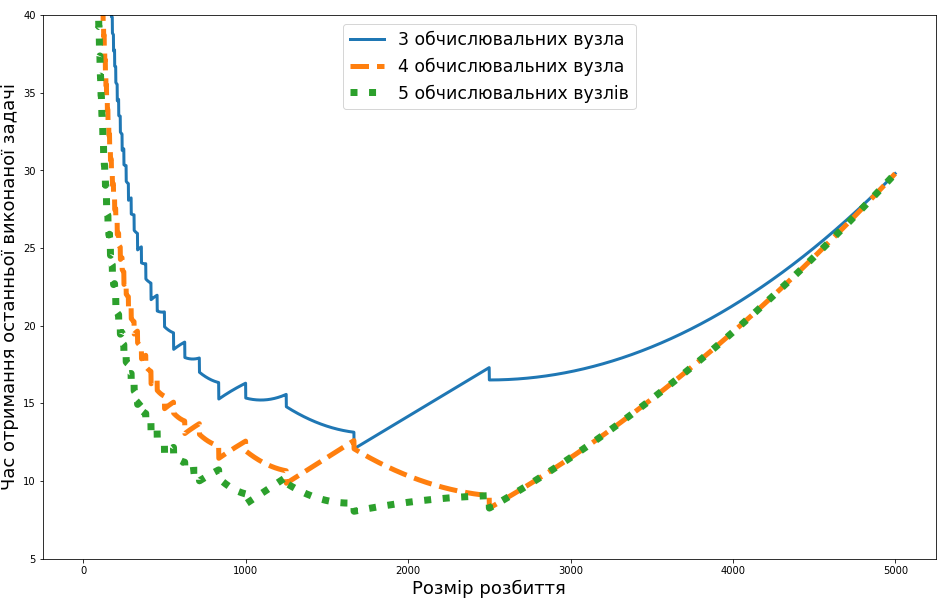
\includegraphics[width=\textwidth]{practice/img/one_user_different_proc}
	\caption{Графік залежності часу виконання всіх задач користувача від розміру розрізання для різних кількостей обчислювальних вузлів}
	\label{fig:one_diff_proc}
\end{figure}

На Рис. \ref{fig:one_diff_N} показано для розмірів матриць 3000, 4000 та 5000 графіки залежності часу виконання усіх задач користувача від розбиття для 5 ОВ. З нього відносно можна помітити, що графіки мають приблизно однакову форму і можливо між ними має місце звичайна пропрорційну залежність від розміру матриці N.

\begin{figure}[H]
	\centering
	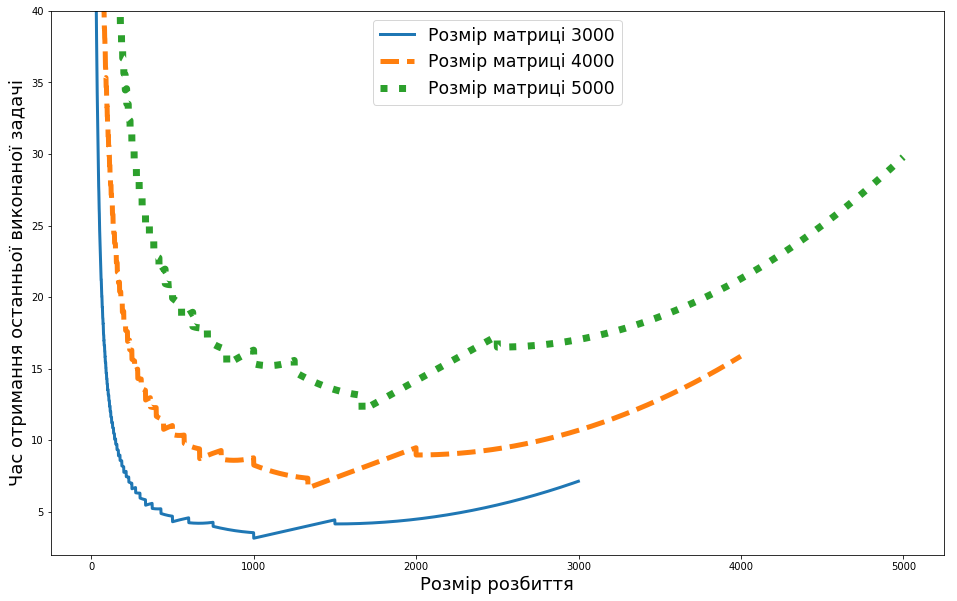
\includegraphics[width=\textwidth]{practice/img/one_user_different_N}
	\caption{Графік залежності часу виконання всіх задач користувача від розміру розрізання для різних розмірів матриць}
	\label{fig:one_diff_N}
\end{figure}

\subsection{Аналіз штрафів за розбиття}

Також варто перевірити аналіз штрафів з теоретичного розділу за допомогою симуляційної системи. Це дуже просто зробити, оскільки програма дозволяє задавати деякі з параметрів як $\inf$. 3 досліджувані параметри це: ping, bandwidth та mips. Якщо поставити $bandwidth=\inf$ та $mips=\inf$, тоді складові часу, які відповідають за передачу даних та саме общичслення, обнуляться і ми будемо мати чисто лише час, який був спричинений затримками пакетів.

Проводити експерименти будемо для конфігурацій із заниженими потужностями обчислювальних 3х вузлів $6e7$ операцій/секунду, малим значенням пропускної здатності $8e7$ біт/секунду та затримкою пакетів в 1 мілісекунду.

Таблиця \ref{table:penlties_table} наглядно показує для випадку множення матриць розмірів 1200 штрафи. Також можемо побачити велику різницю мів розрізаннями $1200$ , $600$ та $400$. $1200$ значить не розрізати матрицю та фактично виконати множення на одному ядрі, також час із першої колонки відповідає за чистий час обчислень без додавання часу пересилки та затримок. Час для розрізання $600$ також ще поганий, оскільки було сформовано 4 задачі у той час як доступні всього 3 обчислювальних вузла. Тобто остання задача виконувалась лише на одному вузлі поки інші простоювали. Далі починаючи з розрізання $400$ час відносно стабілізується. Це можна пояснити тим, що для наступних розрізань хоч і результуюча кількість задач може не бути дільником кількості обчислювальних вузлів, проте задачі вже настільки малі, що час простою в кінці значно менший ніж для випадків $1200$ та $600$. Також ці результати підтверджують теорію про те, що складність множення матриць ніяк не змінюється від щільності розбиття.

\begin{table}[!htbp]
	\centering
	\caption{Таблиця штрафів від величини розрізання}
	\begin{tabular}{c | c | c | c}
		
		\csvautotabular{practice/csv/data_together_p_0.001_bw_8e7_mips_6e7.csv}
		
	\end{tabular}
	\label{table:penlties_table}
\end{table}

Розглянемо окремо графіки трьох складових загального часу (Рис.\ref{fig:three_types_penalties}): виконання задач, передачі даних та затримок.

\begin{figure}[H]
	\centering
	\begin{subfigure}[b]{0.5\linewidth}
		\centering
		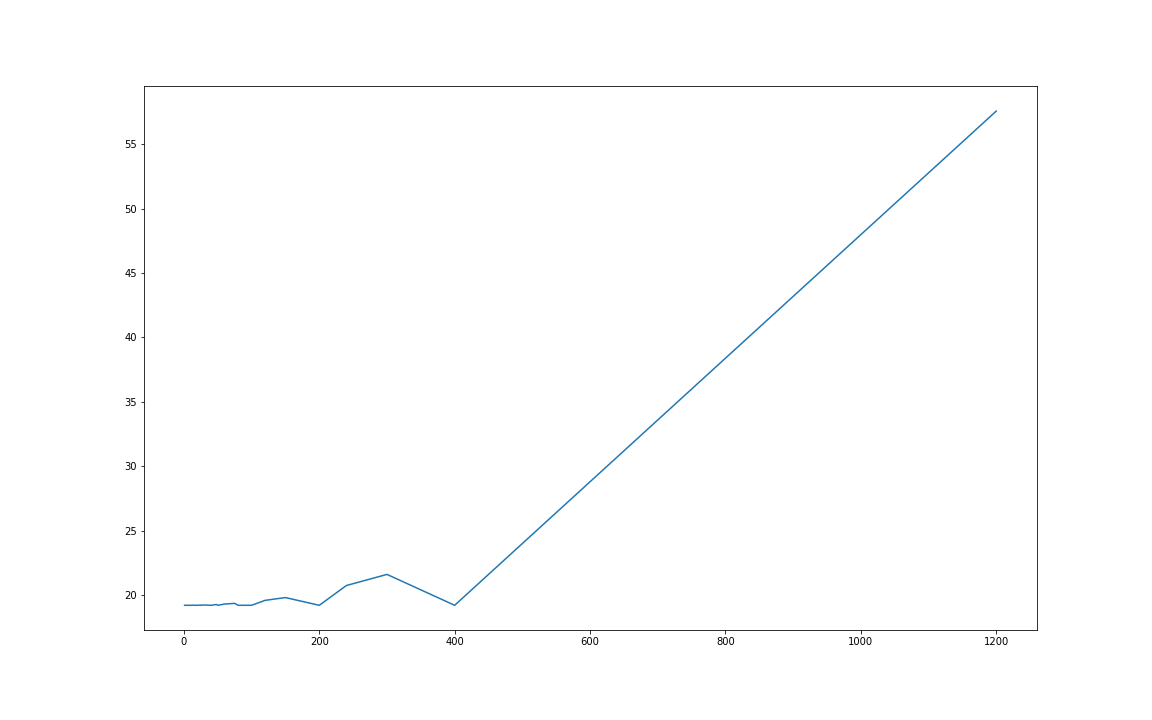
\includegraphics[width=\textwidth]{practice/img/processing_time_sep}
		\caption{Графік часу обчислень від розміру розрізання}
		\label{fig:processing_time_sep}
	\end{subfigure}%

	\begin{subfigure}[b]{0.5\linewidth}
		\centering
		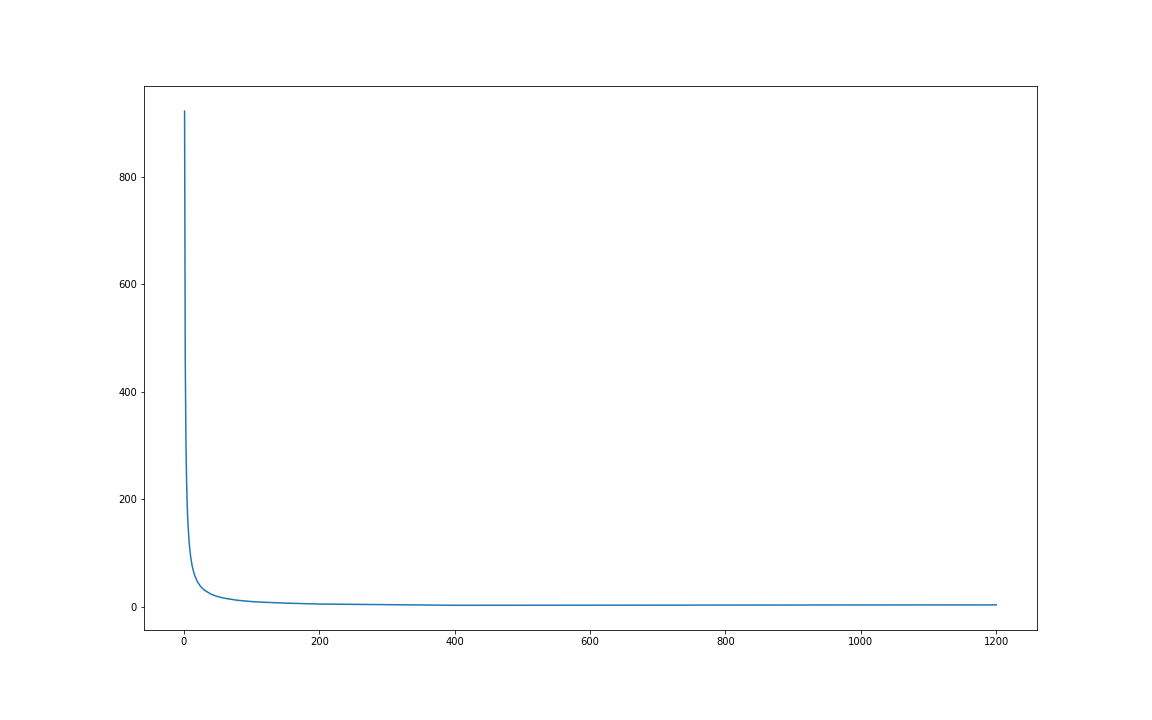
\includegraphics[width=\textwidth]{practice/img/transfer_time_sep}
		\caption{Графік часу передачі даних від розміру розрізання}
		\label{fig:transfer_time_sep}
	\end{subfigure}\\

	\begin{subfigure}[b]{0.5\linewidth}
		\centering
		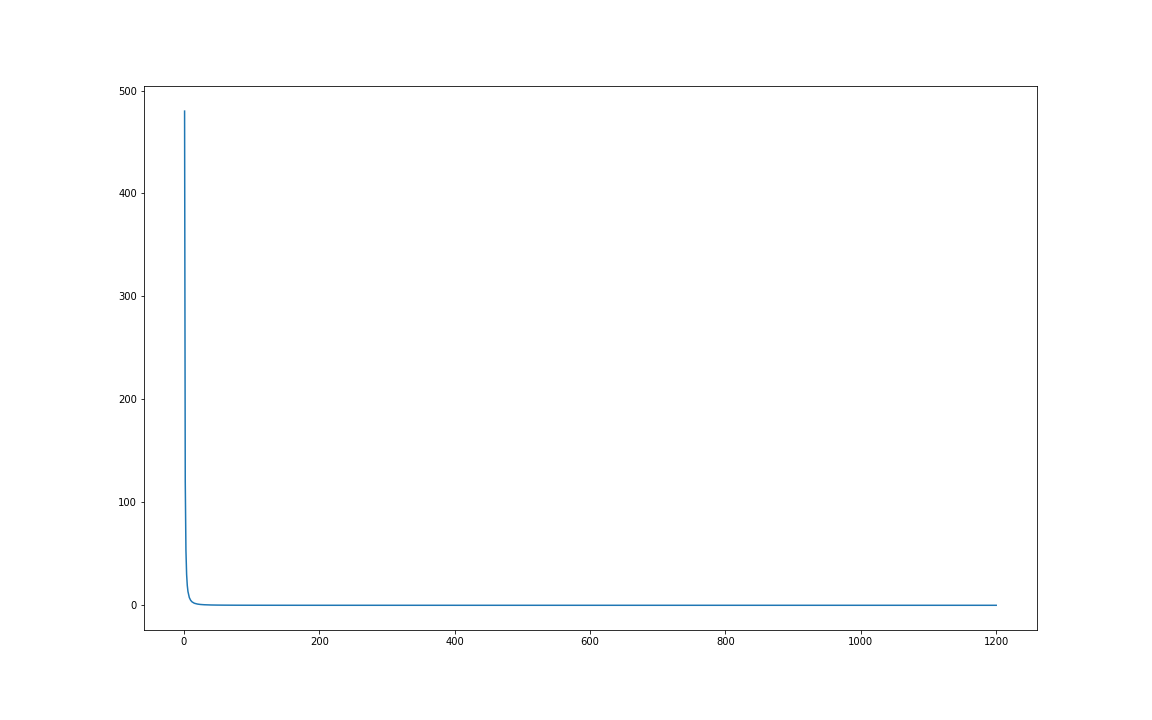
\includegraphics[width=\textwidth]{practice/img/latency_time_sep}
		\caption{Графік часу затримок від розміру розрізання}
		\label{fig:latency_time_sep}
	\end{subfigure}
	\caption{Графіки трьох типів штрафів окремо}
	\label{fig:three_types_penalties}	
\end{figure}

\subsection{Симуляція для двої користувачів}

На Рис. \ref{fig:two_users_fixed_first} зображено залежність часу виконання усіх задач другого користувача від розміру розбиття при фіксованому розбитті користувача 1 для 5 ОВ. На графіку чітко спостерігається стрибки при переході розбиття користувача 2 за фіксоване значення розбиття користувача 1. Це особливість minmin та minmax оскільки вони в першу чергу виконують найлегші задачі, тому користувач, що вибрав менше розбиття, має менший час виконання усіх його задач.

\begin{figure}[H]
	\centering
	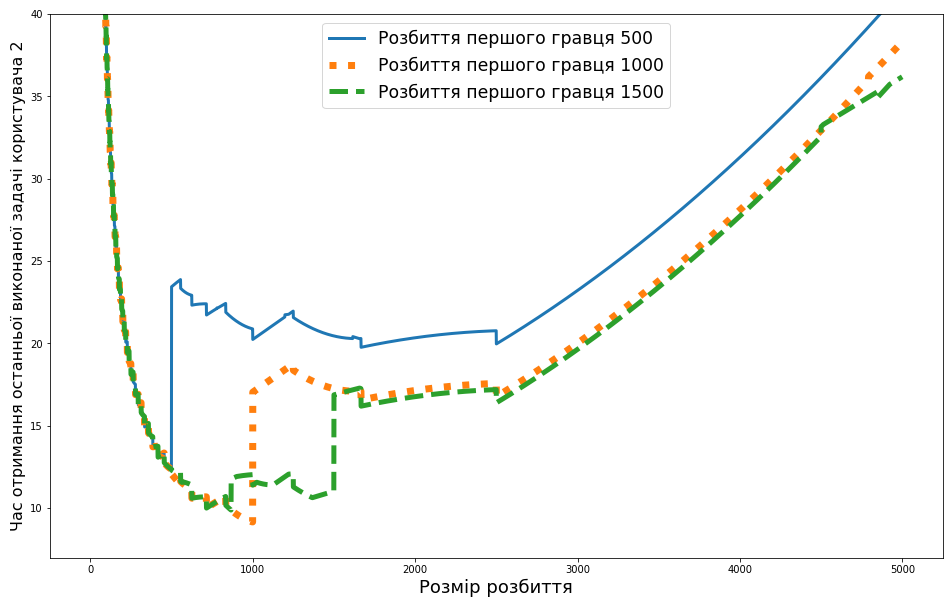
\includegraphics[width=\textwidth]{practice/img/two_users_fixed_first}
	\caption{Графік залежності часу виконання всіх задач другого користувача від розміру його стратегії розрізання при фіксованих стратегіях першого користувача}
	\label{fig:two_users_fixed_first}
\end{figure}

На перший погляд поверхя, яка отримана шляхом симуляції усіх можливих пар стратегій обох користувачів з відріка $[20, 400]$, може здааватися гладкою та випуклою Рис. \ref{fig:two_users_surface_plot_20_400}. Проте, пам'ятаючи природу графіків при фіксованій стратегії першого користувача на Рис. \ref{fig:two_users_fixed_first}, слід подивитися на Рис. \ref{fig:two_users_surface_plot_20_400} більш ретельно, наприклад побудувати поверхню усіх комбінацій стратегій з відрізка $[150, 350]$.

\begin{figure}[H]
	\centering
	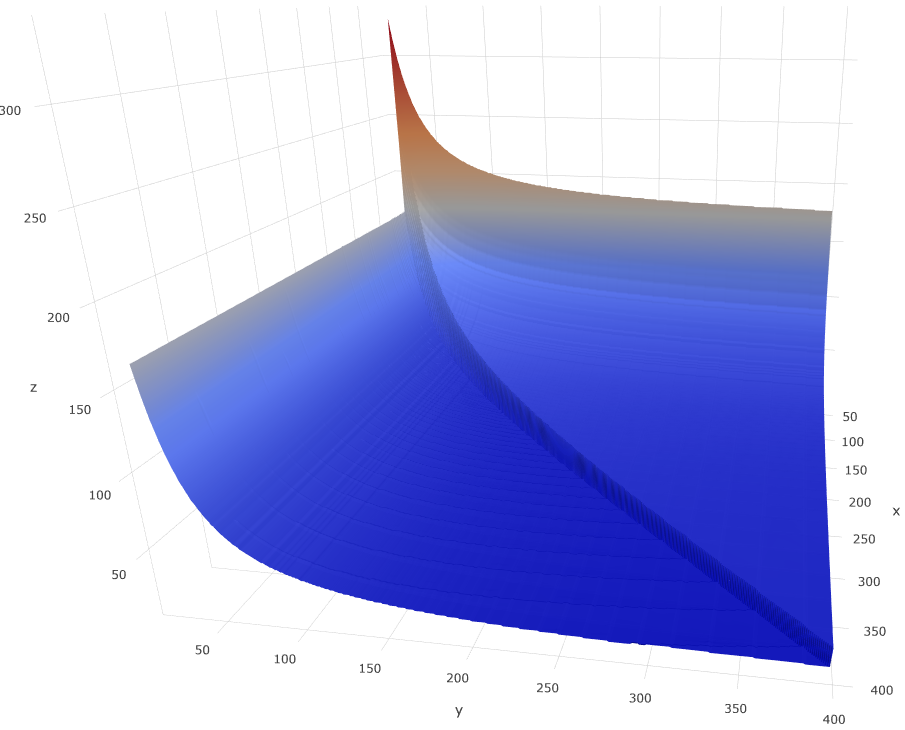
\includegraphics[width=\textwidth]{practice/img/two_users_surface_plot_20_400}
	\caption{Графік залежності часу виконання всіх задач другого користувача для всіх комбінацій стратегій обох користувачів з відрізка $[20, 400]$}
	\label{fig:two_users_surface_plot_20_400}
\end{figure}

При кращій деталізації можна чітко побачити, що на Рис. \ref{fig:two_users_surface_plot_150_350_top} спостерігається форма сходинок по всій верхній частині графіка і вона не така проблемна, як нижня частина, показана на Рис. \ref{fig:two_users_surface_plot_150_350_bot}. Оскільки нижня частина більш цікава через те, що час завершення усіх задач користувача там менший, то і глобальний мінімум варто шукати саме на нижній частині. Нижня частина має особливої форми канави і саме вони є основною проблемою.

\begin{figure}[H]
	\centering
	\begin{subfigure}[b]{0.45\textwidth}
		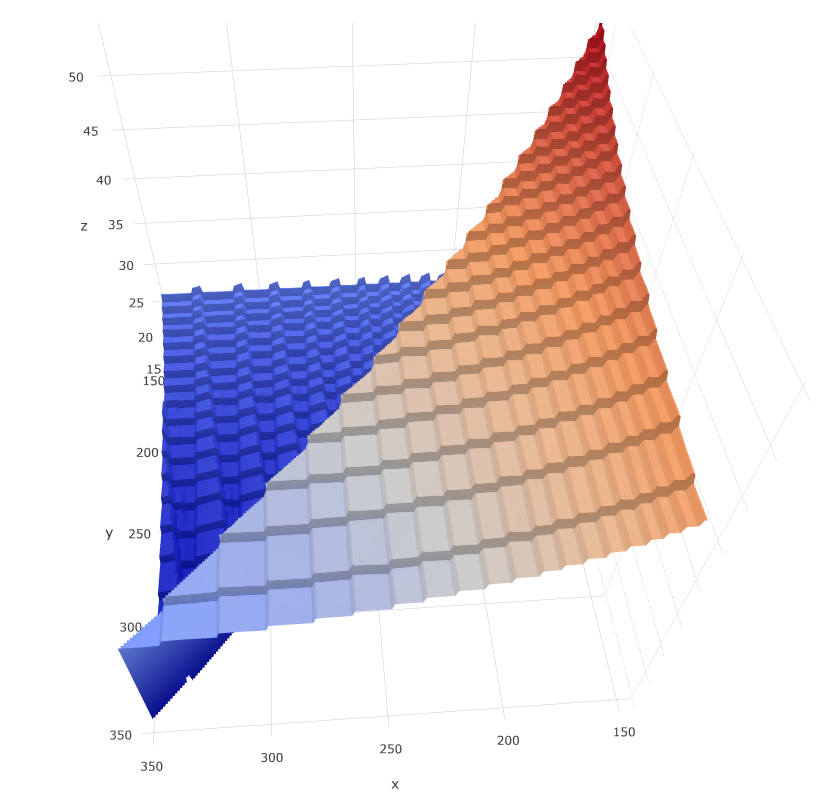
\includegraphics[width=\textwidth]{practice/img/two_users_surface_plot_150_350_top}
		\caption{Верхня частина графіка}
		\label{fig:two_users_surface_plot_150_350_top}
	\end{subfigure}
	\hfill
	\begin{subfigure}[b]{0.45\textwidth}
		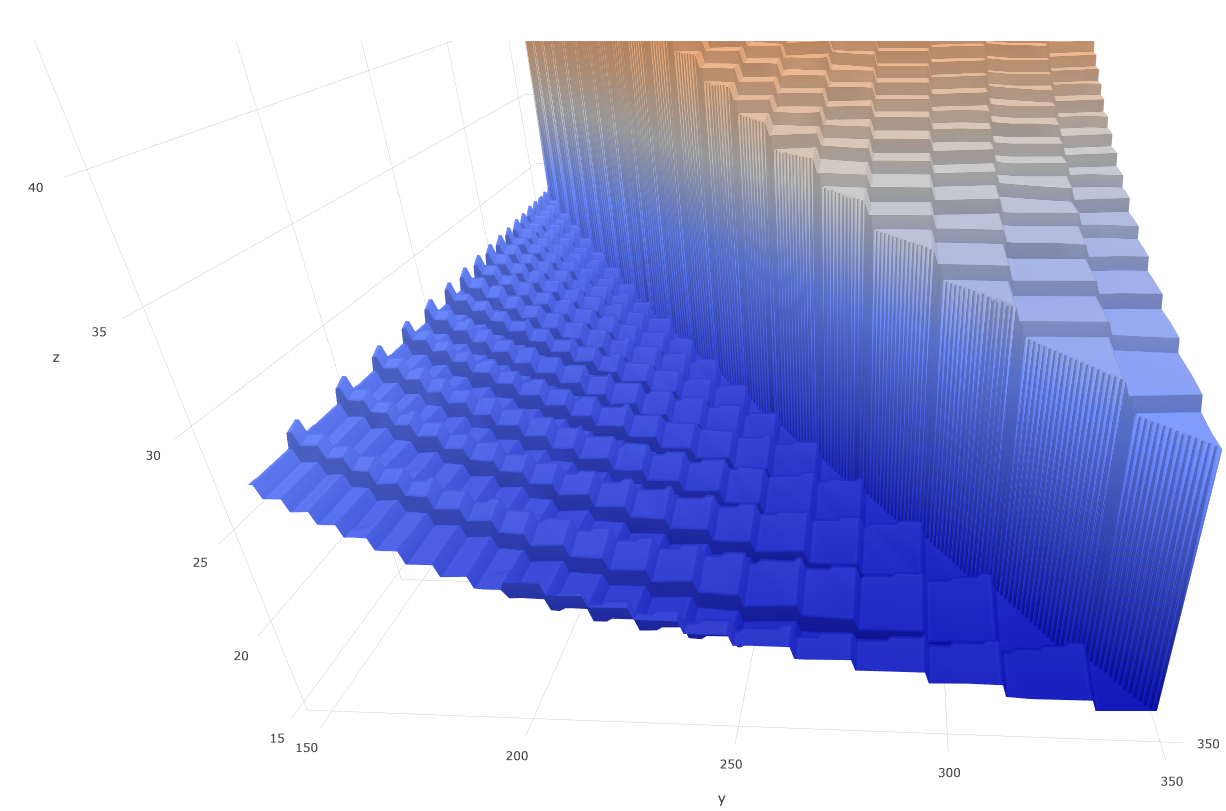
\includegraphics[width=\textwidth]{practice/img/two_users_surface_plot_150_350_bot}
		\caption{Нижня частина графіка}
		\label{fig:two_users_surface_plot_150_350_bot}
	\end{subfigure}
	\caption{Графік залежності часу виконання всіх задач другого користувача для всіх комбінацій стратегій обох користувачів з відрізка $[150, 350]$, \ref{fig:two_users_surface_plot_150_350_top} - фокус на верхню частину поверхні, \ref{fig:two_users_surface_plot_150_350_bot} - фокус на нижню частину поверхні}
	\label{fig:two_users_surface_plot_150_350}
\end{figure}

З Таблиці \ref{table:values_table} можна побачити як в між деякими сусідніми значеннями спочатку час трохи збільшується, а потім різко зменшується. Таким чином структура функції і проблеми її оптимізації очевидні.

\begin{table}[H]
	\centering
	\caption{Таблиця значень часів повернення усіх задач користувачів для різних стратегій розрізань}
		\begin{tabular}{c | c | c | c}
			\csvautotabular{practice/csv/5000_min_min_proc3_p0.0_bw1e9.csv}
		
		\end{tabular}
	\label{table:values_table}
\end{table}

\section{Застосування оптимізації до знаходження мінімуму}

Спробуємо застосувати метод оптимізації з метою спуску до мінімуму. Перевіримо, що в залежності від початкової точки оптимізація буде застрягати у локальному мінімумі.

Застосуємо звичайний по координаті, яка зменшує час більше всього і запустимо його ітеративно.

На виході з симуляційної системи ми отримуємо квадратну матриці для обох гравців з їх часами отримання усіх задач. Позначимо їх так само як і у теоретичному розділі за $A,B \in \mathbb{R}^{N*N}$ як програші гравців 1 та 2 відповідно. Проте оскільки ми знаемо, що матриці при багаторазовому повторені експерименту та усереднені результатів, такі, що $A=B^T$. То будемо розглядати оптимізацію часу лише одного гравця, наприклад першого.

Нехай задана початкова точка $(a_0, b_0)$ як початкові стратегії користувачів. З цієї точки стартує алгоритм.

Етапи роботи алгоритма спуску:
\begin{itemize}
	\item[1.] Задаємо початкову точку $p_0 = (a_0, b_0)$, час у точці $p_0$ поставимо за $t_0 = A_{a_0 b_0}$. Поставимо k=0.
	\item[2.] Шукаємо найменший час по квадрату зі сторонами в 3 елементи матриці і центром у точці $p_k$.
	\item[3.] Вибираємо точку з найменшим часом та ставимо її як $p_{k+1}$. Якщо $p_{k+1}=p_{k}$, то зупиняємо алгоритм.
	\item[4.] $k=k+1$, повертаємося на крок 2.
\end{itemize}

Перевіримо як працює алгоритм. Для перевірки проведемо симуляцію для розміру матриць 10000 по розрізанням, які є дільниками 10000, нехтуємо розширенням симуляцій з блоками. Знайдемо глобальний мінімум та спробуємо запустити оптимізацію з різних стартових точок. Потужності обчислювальних вузлів поставимо у співвідношенні 2:2:1. Тобто три обчислювальних вузла.

Як бачимо з таблиці \ref{table:optimize_results}, оптимізація працює непогано в сенсі що дозволяє вибратись з неефективних точок. Проте оптимізація застрагяє і не доходить до глобального мінімума. І як ми пам'ятаемо за Рис. \ref{fig:two_users_surface_plot_150_350}, при розгорнутій симуляції з розбиттями, які не є дільниками розмірності матриці, то там канави зустрічаються дуже часто, що говорить про повну неможливість використовувати методи оптимізації для знаходження оптимальної точки, проте у випадку дільників розмірності матриці оптимізація допомагає вибратись з поганих точок до відносно хороших, які по часу дуже близько до глобального мінімума.

\begin{table}[H]
	\caption{}
	\label{table:optimize_results}
	\begin{tabular}{|l|l|l|l|l|}
		\hline
		№ & Початкова стратегія & Початковий час 	& Кінцева стратегія & Кінцевий час
		\\ \hline
		1.& (2,2)				& 6670.72055426     &(1250, 2000) 		& 11.0248749
		\\ \hline
		2.& (10000,10000)		& 14.65571875   	&  (5000,10000)		& 13.7184062
		\\ \hline
		3.& (5,25)				& 1335.36618371		&  (1000,1250)		& 11.0248749
		\\ \hline
		4.& (25,5)				& 1604.09384557		&  (1000,1250)		& 11.0248749
		\\ \hline
		5.& (25,5)				& 1604.09384557		&  (1000,1250)		& 11.0248749
		\\ \hline
		6.& (625,40)			& 184.069188072		&  (1000,1250)		& 11.0248749
		\\ \hline
		
	\end{tabular}
\end{table}
